\section{Gradient/PSF approximation for distributed deconvolution} \label{gradients}
For a distributed deconvolution, we would like to deconvolve the image with as little communication as possible. This largely depends on the size of the $PSF$ when compared to the overall image. If the $PSF$ is for example $\frac{1}{16}$ of the total image size, we have patches of the image which are completely independent of each other. Sadly, this is not true for radio interferometers. The $PSF$ is generally the same size as the image. We cannot deconvolve any part of the image independently of each other.

However, we have two effects of modern radio interferometers, that produce an "approximately" smaller $PSF$: First, we have an increasing number of visibilities. They create a $PSF$ that increasingly resembles a Gaussian function in the center, and the rest approaches zero. And secondly, we reconstruct images with a wide field-of-view. Although the $PSF$ is not zero the further away we move from the center, its values approach zero.

\begin{figure}[h]
	\centering
	\begin{subfigure}[b]{0.4\linewidth}
		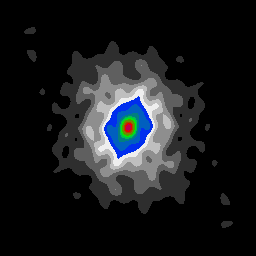
\includegraphics[width=\linewidth]{./chapters/03.distribution/simulated/psf.png}
	\end{subfigure}
	\begin{subfigure}[b]{0.4\linewidth}
		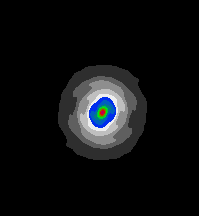
\includegraphics[width=\linewidth]{./chapters/06.gradient/psf_cut.png}
	\end{subfigure}
	
	\caption{$PSF$ arising from an increasing number of visibilities.}
\end{figure} 

In short, with an ever increasing number of visibilities and field-of-view, the influence of far-away image sections become negligible. We can approximate the deconvolution with a fraction of the true $PSF$. To our knowledge, we are the first to propose such approximation methods. In this Section, we present our approximation methods. In Section \ref{results:gradients}, we empirically demonstrate the validity of our approximations on a real-world MeerKAT observation. In Section \ref{pcdm}, we show more sophisticated coordinate descent methods that can exploit the smaller $PSF$. 

\subsection{Intuition behind approximating the $PSF$}

In our coordinate descent deconvolution, we use the $PSF$ in two steps. Before we run coordinate descent, we pre-calculate the gradient for each pixel with a correlation operation. During coordinate descent deconvolutions, we update the gradient-map directly. Two opposing solutions: We use the full $PSF$ to pre-calculate the gradients, but only update the gradients with a fraction of the $PSF$. That way we always start from the correct gradients, but get less accurate over coordinate descent deconvolutions.

\subsection{Method 1: Approximate gradient update}

So we use the full $PSF$

only update with a fraction of the $PSF$

$PSF$ squared update. Scaling.
So we become less and less accurate


\subsection{Method 2:Approximate deconvolution}

We never use the full PSF

But the problem of gradient magnitude. 

Change lambda. We do an approximate deconvolution. 


\subsection{Major Cycle convergence}\label{gradients:pathreg}
\cite{clark1980efficient} and the question on how many iterations per major cycle
Putting it all together

We have the Minor Cycle, which is easy to converge.

Coordinate Descent Path optimization \cite{friedman2010regularization}
Danger that CD takes too many pixel into a Major Cycle. Lower bound per iteration, PSF sidelobe
can still be too low, danger when many psf sidelobes overlap